
% \section{Hardware Implementation}
	\subsection{Overview and objectives}
	
	MD5 is a simple algorithm to implement, however it takes time to find calculate the hash.  Using a Field Programmable Gate Array (FPGA) we hope to improve the time it takes to create a single hash.  For this assignment a Xilinx XC3S1200E-4FG320 FPGA will be utilized on a Digilent Nexys 2 development board.  The FPGA contains 1200K gates, 19,512 logic cells with a total slice count of 8,672.  ISE 13.4 Project Navigator were used to synthesize the design and ModelSim was used to simulate and test it.  The goal for this implementation is to fully pipeline the design so that for every clock cycle a valid hash will be calculated.

	\subsection{Architecture}
		For the architecture a hierarchical implementation was chosen.  The basic building blocks of the design include reg32\_top and add32.  Reg32\_top synthesizes a D-flip flop on the FPGA and add32 synthesizes a 32 bit adder.  These are organized as can be seen in Figure \ref{fig:Round}.  The inputs for each round are : A, B, C, D, K, T, RESET and CLK.  The outputs are : A\_OUT, B\_OUT, C\_OUT and D\_OUT.
\begin{figure}[h]
\centering
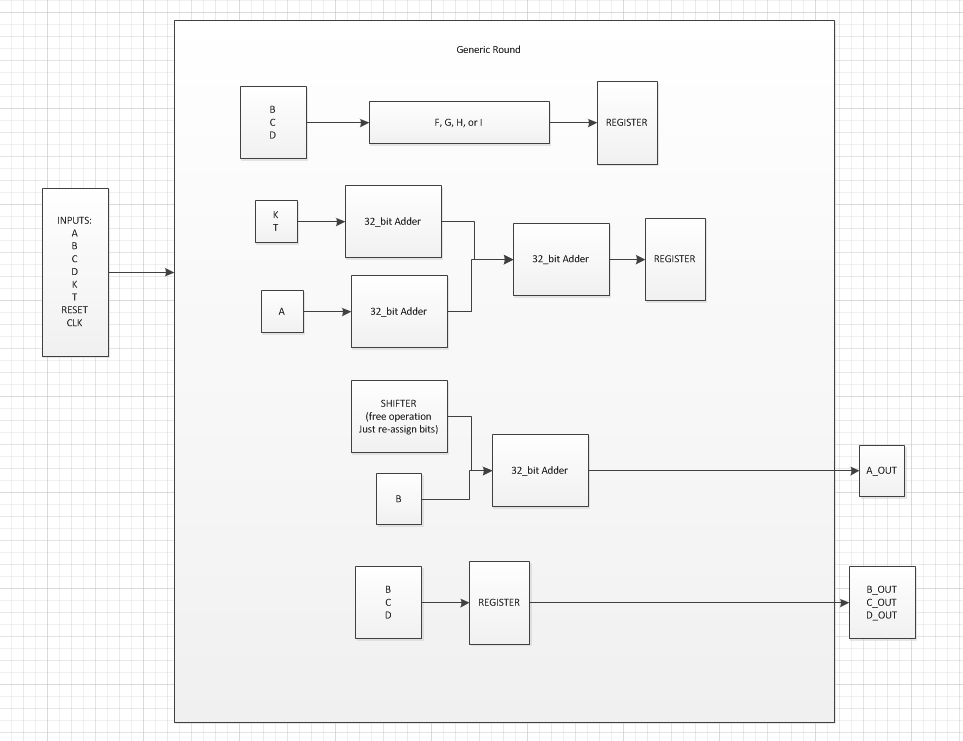
\includegraphics[width=0.7\linewidth]{./Round}
\caption{Generic Round Block Diagram.}
\label{fig:Round}
\end{figure}

		For the top level hierarchy, this generic round is implemented 64 times - 16 times for each of the functions: F, G, H, and I.  Then after these 64 cycles the outputs are added to the initial values to complete the MD5 hash algorithm.  The top level block diagram can be seen in Figure \ref{fig:Top}.
\begin{figure}[h]
\centering
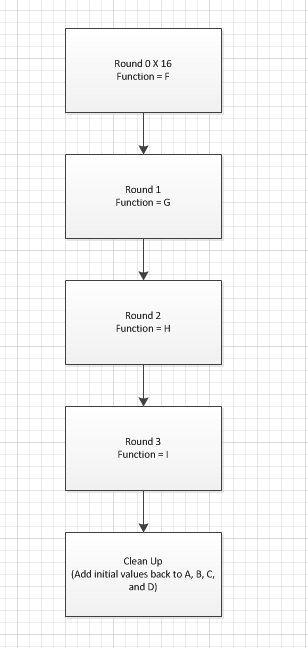
\includegraphics[width=0.7\linewidth]{./Top}
\caption{Top Level Block Diagram.}
\label{fig:Top}
\end{figure}
	\subsection{Benchmarking}
		The final benchmarking of this design was straightforward.  It was determined using the performance equation : Throughput = (Block size * Clock Frequency)/(Cycles per block).  The block size was 1, the clock frequency was up to 115MHz and the cycles per block was 1 so filling those numbers into the equation : (1*115Mhz/1) = 115 Mega Hashes per second.  The maximum clock frequency was derived from the report given by Project Navigator that the best case achievable clock period was 8.680ns.  1/8.680ns = 115MHz.
	\subsection{Performance}
		The performance achieved was decent when thought of in hashes per dollar.  The Nexsys 2 board can be purchased from Digilent for \$200.00.  115 Megahashes per second divided by the cost of the board yields 0.575 Megahashes per dollar or 5750 hashes per cent.  This is much less costly than implementing it on a computer which can cost several hundreds of dollars more.  
		
		Higher performance can be achieved by procuring a larger FPGA.  It is very simple to improve performance.  All that is needed is to implement the same design multiple times on a larger FPGA and your performance is improved proportionate to the number of implementations instantiated.  Another way is to increase clock speed on a different FPGA which can support it, or purchase the same FPGA with a greater speed grade.
		
		The total gate count has been removed from the Xilinx design tools after the release of 10.1 so flip flops, 4 input LUTs and slices will be discussed instead.  The FPGA used has a total number of 12,344 flip flops, of which, 12,044 were used or 69\%,  7,588 of the available 17,344 4 input LUTs were used or 43\% and 7,202 of the available 8,672 slices were occupied or 83\%\cite{fpga}.  Each slice contains two LUTs and two flip-flops.  As can be seen, if the number of registers could have been reduced to under 50\%, perhaps two top-level entities could have fit within the design.  However, as I reduced the number of register, or pipeline stages, the maximum clock frequency rapidly decreased. The fully pipelined design yielded the  highest hash rate.
	

